% Compile with lualatex

\PassOptionsToPackage{unicode}{hyperref}
\documentclass[aspectratio=1610,9pt]{beamer}

\usepackage[english]{babel}
\usepackage{csquotes}
\usepackage{amsmath}
\usepackage{amssymb}
\usepackage{mathtools}
\usepackage{siunitx}
\usepackage{graphicx}
\usepackage{hyperref}
\usepackage{bookmark}
\usepackage[percent]{overpic}
\usepackage{xcolor}

\usetheme[
  showtotalframes,
]{tudo}

\sisetup{
  separate-uncertainty = true,
  per-mode = symbol,
}

\unimathsetup{
  math-style=ISO,
  bold-style=ISO,
  nabla=upright,
  partial=upright,
  mathrm=sym,
}

\title{Discovery of a Radiation Component from the Vela Pulsar Reaching \texorpdfstring{\qty{20}{\tera\electronvolt}}{20 TeV}}
\author{Akram Aki}
\institute{Neutrino and Gamma-ray Astronomy Seminar}
\date{SS 2026}

\begin{document}

\begin{frame}[plain]
  \noindent\makebox[\paperwidth][l]{%
    \hspace*{-0.54cm}%
    \vspace*{-1cm}%
    \begin{overpic}[width=\paperwidth, keepaspectratio]{images/vela_region.png}
      % Zoom image
      \put(20,20){
        \fcolorbox{red}{black}{%
          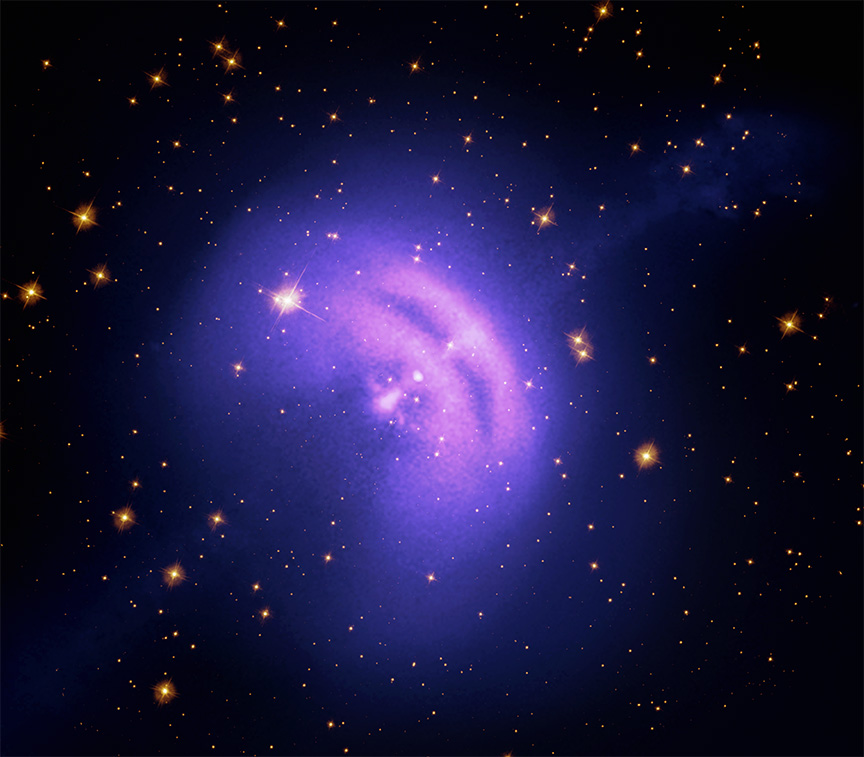
\includegraphics[width=0.25\paperwidth]{images/vela_zoom.png}
        }
      }

      \color{red}
      \linethickness{0.5pt}

      % upper connection line
      \qbezier(58.5,29)(50,40)(47.2,42.5)

      % lower connection line
      \qbezier(58.2,24.5)(50,20)(47.2,19.5)

      % Title text
      \put(50,55){%
        \makebox(0,0){%
          \begin{minipage}{0.78\paperwidth}
            \centering
            \color{white}
            \Huge\bfseries
            Discovery of a Radiation Component\\[0.25em]
            from the Vela Pulsar Reaching\\[0.25em]
            \qty{20}{\tera\electronvolt}
          \end{minipage}
        }%
      }
    \end{overpic}%
  }
\end{frame}

\begin{frame}{Why is the Vela pulsar interesting?}
  \begin{columns}[T,onlytextwidth]
    \begin{column}{0.52\textwidth}
      \vspace{0.3cm}
      \begin{itemize}
        \item A young neutron star inside the Vela supernova remnant
        \item One of the brightest persistent sources in the gamma-ray sky
        \item Rotates once every \qty{89}{\milli\second}
        \item H.E.S.S. detects pulsed emission up to \qty{20}{\tera\electronvolt}
      \end{itemize}

      \vspace{0.5cm}

      \begin{block}{Guiding question}
        Why is pulsed emission at \qty{20}{\tera\electronvolt}
        difficult to explain with standard pulsar-emission models?
      \end{block}
    \end{column}

    \begin{column}{0.44\textwidth}
      \centering
      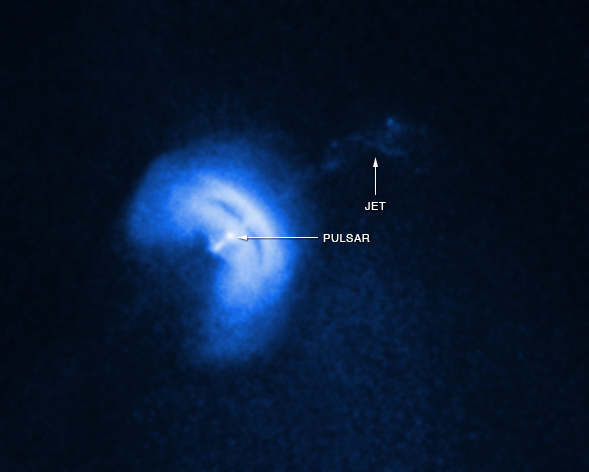
\includegraphics[width=\textwidth]{images/vela_pulsar_context.png}

      \vspace{0.15cm}
      {\scriptsize Vela pulsar and surrounding nebula / remnant}
    \end{column}
  \end{columns}
\end{frame}
% Sources up to this point https://chandra.harvard.edu/deadstar/vela.html

\begin{frame}{From a dead star to a neutron star}
  \begin{columns}[T,onlytextwidth]
    \begin{column}{0.48\textwidth}
      \vspace{0.25cm}
      \begin{itemize}
        \item Massive stars end their lives in a core-collapse supernova
        \item The central remnant can become a neutron star
        \item Typical radius: only about \qty{10}{\kilo\meter} to \qty{15}{\kilo\meter}
        \item Enormous density, rapid rotation, and strong magnetic fields
      \end{itemize}

      \vspace{0.45cm}

      \begin{block}{Key idea}
        Collapse does not just make the object smaller:
        it turns the remnant into an extreme rotating electromagnetic system.
      \end{block}
    \end{column}

    \begin{column}{0.48\textwidth}
      \centering
      %https://en.wikipedia.org/wiki/Neutron_star
      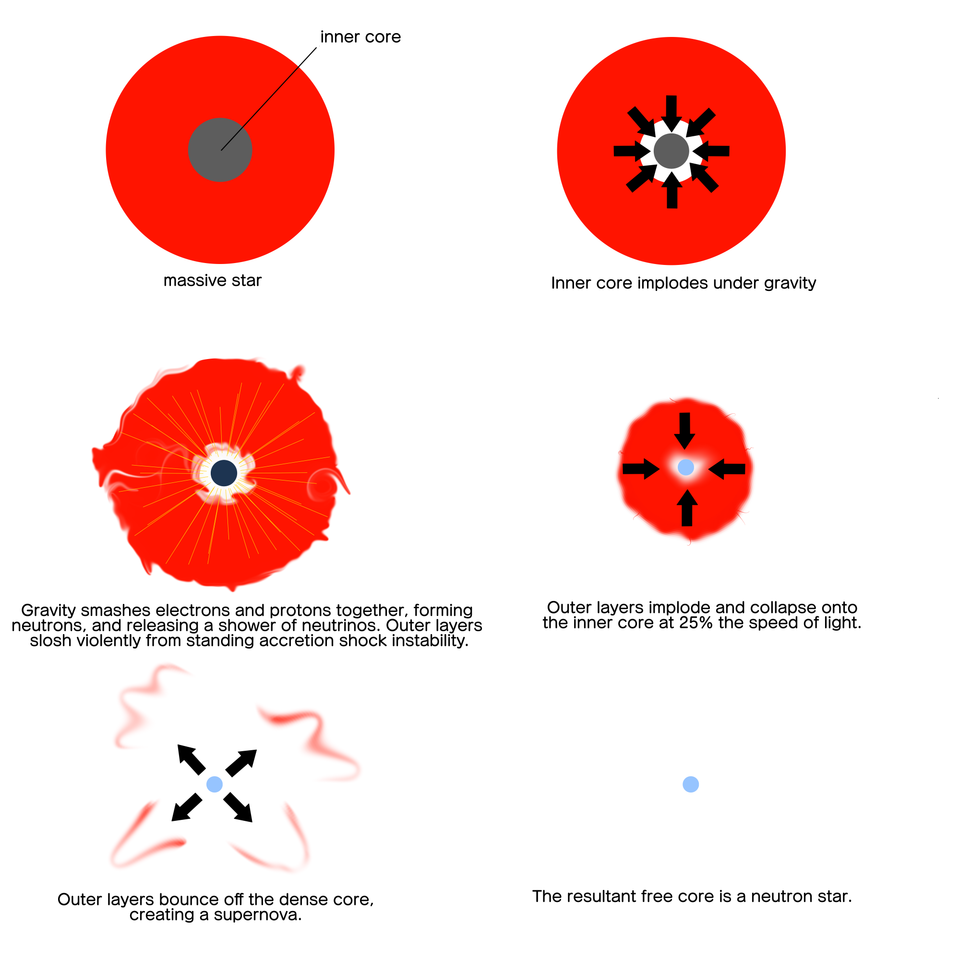
\includegraphics[width=\textwidth]{images/core_collapse_neutron_star.png}

      \vspace{0.15cm}
      {\scriptsize Schematic evolution from massive star to neutron star}
    \end{column}
  \end{columns}
\end{frame}

\begin{frame}{Collapse creates an extreme environment}
  \begin{columns}[T,onlytextwidth]

    \begin{column}{0.58\textwidth}
      \centering
      %https://www.cv.nrao.edu/~sransom/web/Ch6.html
      \vspace*{-0.35cm}
      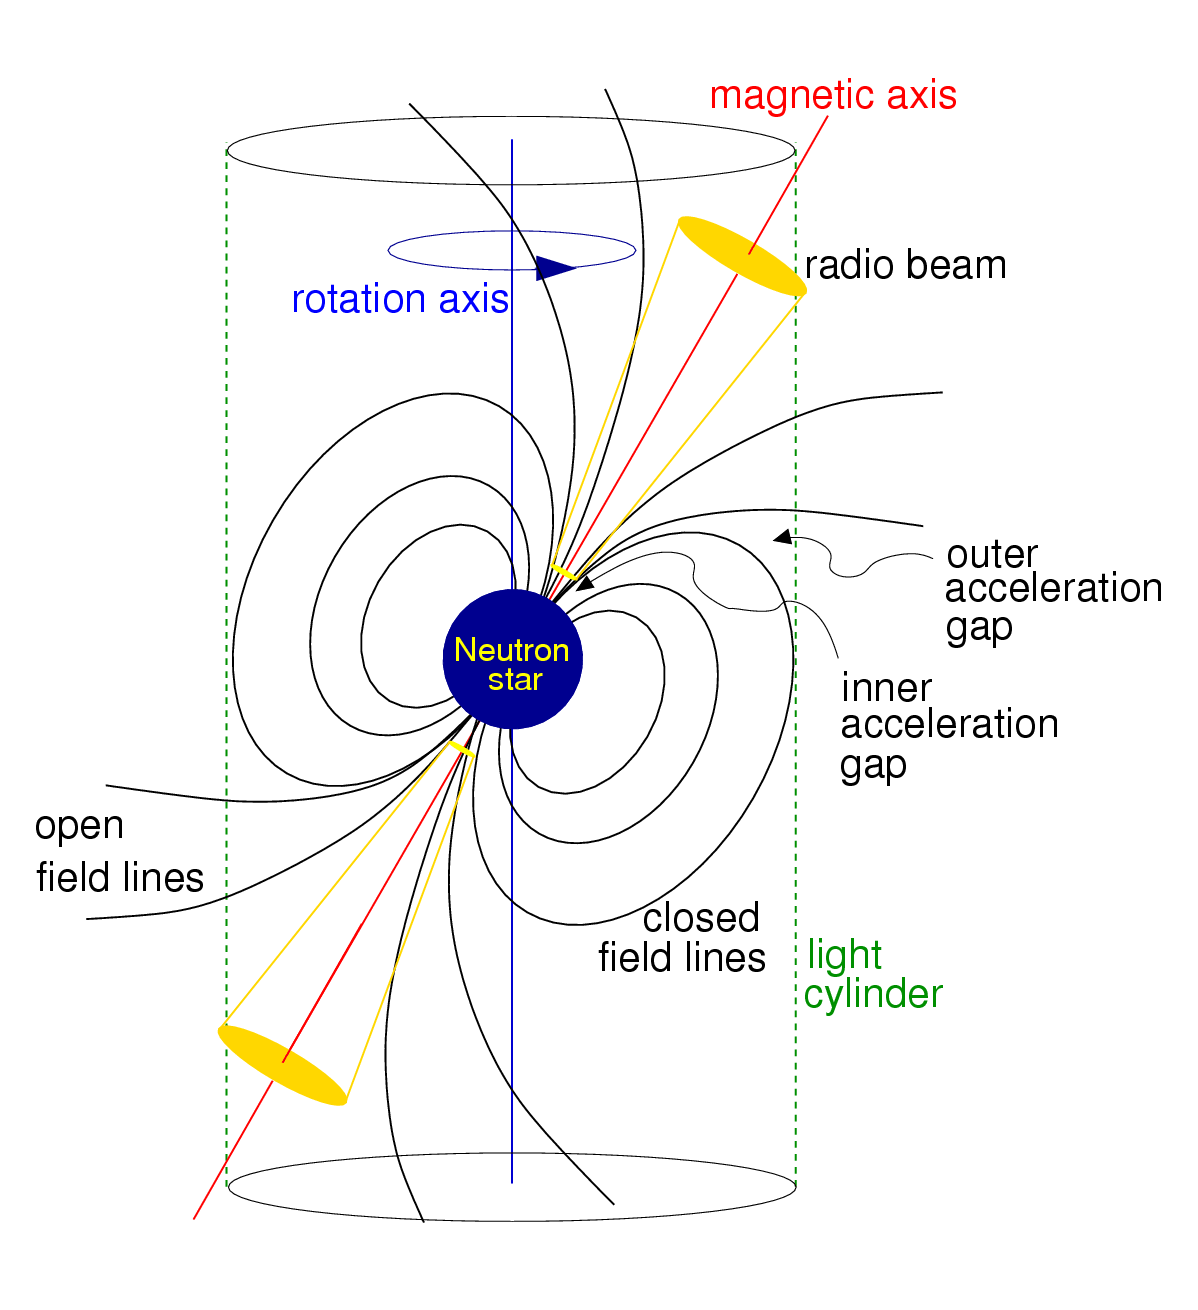
\includegraphics[height=\textheight, keepaspectratio]{images/neutron_star_fieldlines.png}
    \end{column}

    \begin{column}{0.38\textwidth}
      \vspace{0.5cm}

      \begin{itemize}
        \item Radius:
        \qtyrange{10}{15}{\kilo\meter}

        \vspace{0.3cm}

        \item Vela rotates about
        \qty{11}{times\per\second}

        \vspace{0.3cm}

        \item Magnetic fields up to
        \qty{e8}{\tesla}
      \end{itemize}

      \vspace{0.6cm}

      \begin{block}{Key idea}
          Extreme electromagnetic conditions enable efficient particle acceleration.
      \end{block}
    \end{column}

  \end{columns}
\end{frame}

\begin{frame}{Charged particles inside the magnetosphere}

  \begin{columns}[T,onlytextwidth]

    \begin{column}{0.54\textwidth}

      \centering
      %https://heasarc.gsfc.nasa.gov/docs/xte/learning_center/xray_techc.html
      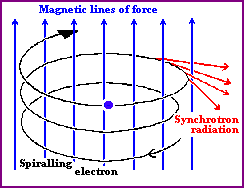
\includegraphics[width=\textwidth]{images/synchrotron_motion.png}

      \vspace{0.15cm}

      {\scriptsize Charged particles spiral around magnetic field lines}

    \end{column}

    \begin{column}{0.42\textwidth}

      \vspace{0.35cm}

      \begin{itemize}

        \item Charged particles are forced onto curved trajectories by magnetic fields

        \vspace{0.25cm}

        \item Stronger magnetic fields reduce the gyration radius

        \vspace{0.25cm}

        \item In pulsars, particles effectively follow the magnetic field structure

        \vspace{0.25cm}

        \item The rotating magnetic field forces approximate co-rotation of the surrounding plasma

        \end{itemize}

        \vspace{0.55cm}

        \begin{block}{Key idea}
            The magnetosphere controls how particles move and where radiation can be produced.
        \end{block}

    \end{column}

  \end{columns}

\end{frame}

\begin{frame}{The light cylinder}
  \begin{columns}[T,onlytextwidth]

    \begin{column}{0.58\textwidth}
      \centering
      % https://www.cv.nrao.edu/~sransom/web/Ch6.html
      \vspace*{-0.35cm}
      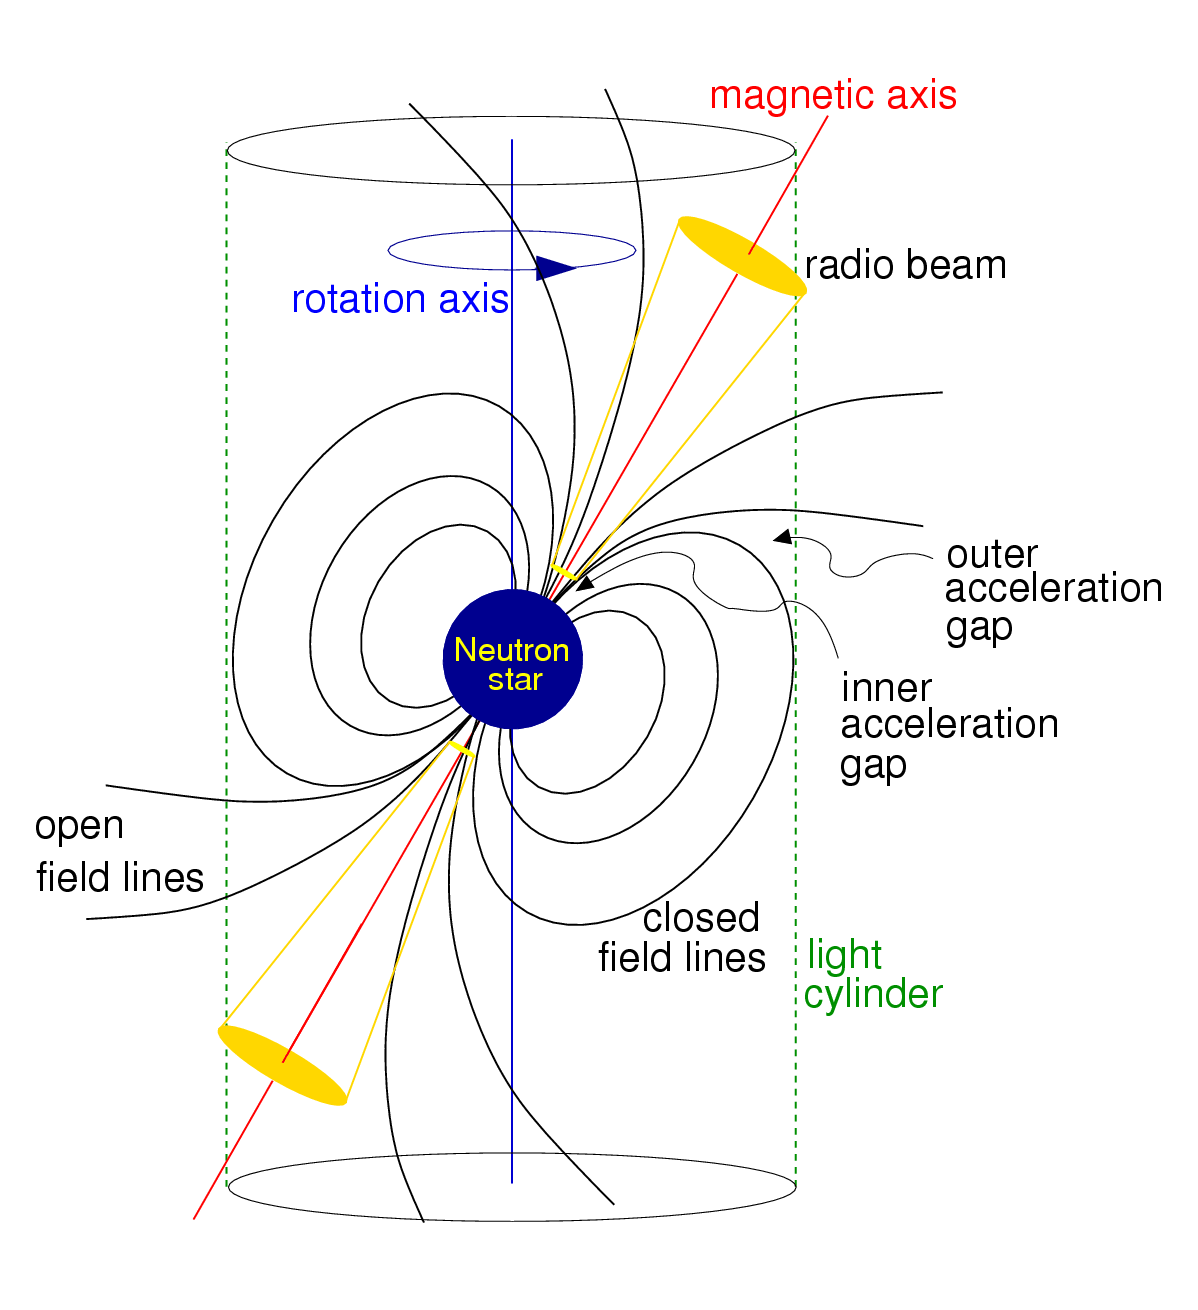
\includegraphics[height=\textheight, keepaspectratio]{images/neutron_star_fieldlines.png}
    \end{column}

    \begin{column}{0.38\textwidth}
      \vspace{0.05cm}

      \begin{block}{From co-rotation to a limit}
        If the magnetosphere co-rotates with the neutron star,
        the linear speed increases with distance from the rotation axis.
      \end{block}

      \vspace{0.15cm}

      \[
        R_{\mathrm{LC}} = \frac{c}{\omega}
      \]

      \vspace{0.2cm}

      \begin{itemize}
        \item At this radius, co-rotation would require the speed of light

        \vspace{0.18cm}

        \item Beyond it, rigid co-rotation is impossible

        \vspace{0.18cm}

        \item Magnetic field lines open up and particles can escape outward
      \end{itemize}

    \end{column}

  \end{columns}
\end{frame}

\begin{frame}{Pulsed emission from neutron stars}

  \begin{columns}[T,onlytextwidth]

    \begin{column}{0.42\textwidth}
      \centering

      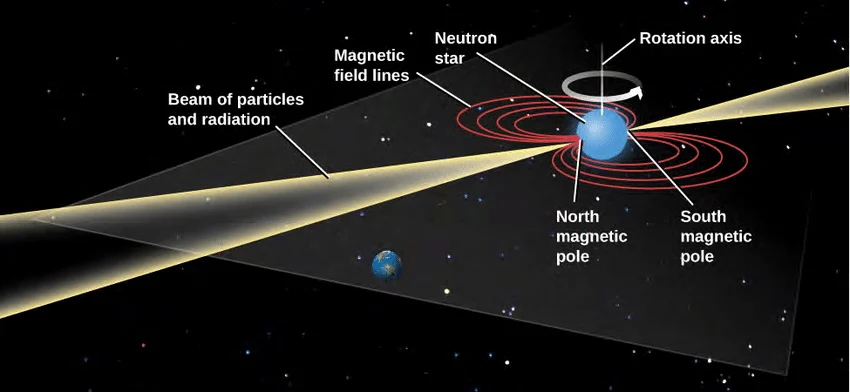
\includegraphics[
        width=\textwidth,
        trim={5cm 3.5cm 3cm 0cm},
        clip
      ]{images/pulsar_beam_schematic.png}

      \vspace{0.08cm}

      {\scriptsize Simplified picture: rotation modulates the observed emission}
    \end{column}

    \begin{column}{0.54\textwidth}
      \vspace{0.25cm}

      \begin{block}{Key idea}
        The observed radiation is connected to the rotating magnetosphere,
        producing characteristic periodic pulse profiles.
      \end{block}

      \vspace{0.2cm}

      {\footnotesize
      The detailed emission geometry is more complex and remains an active
      area of research. Here, only a high-level picture is used.}
    \end{column}

  \end{columns}

  \vspace{0.1cm}

  \centering

  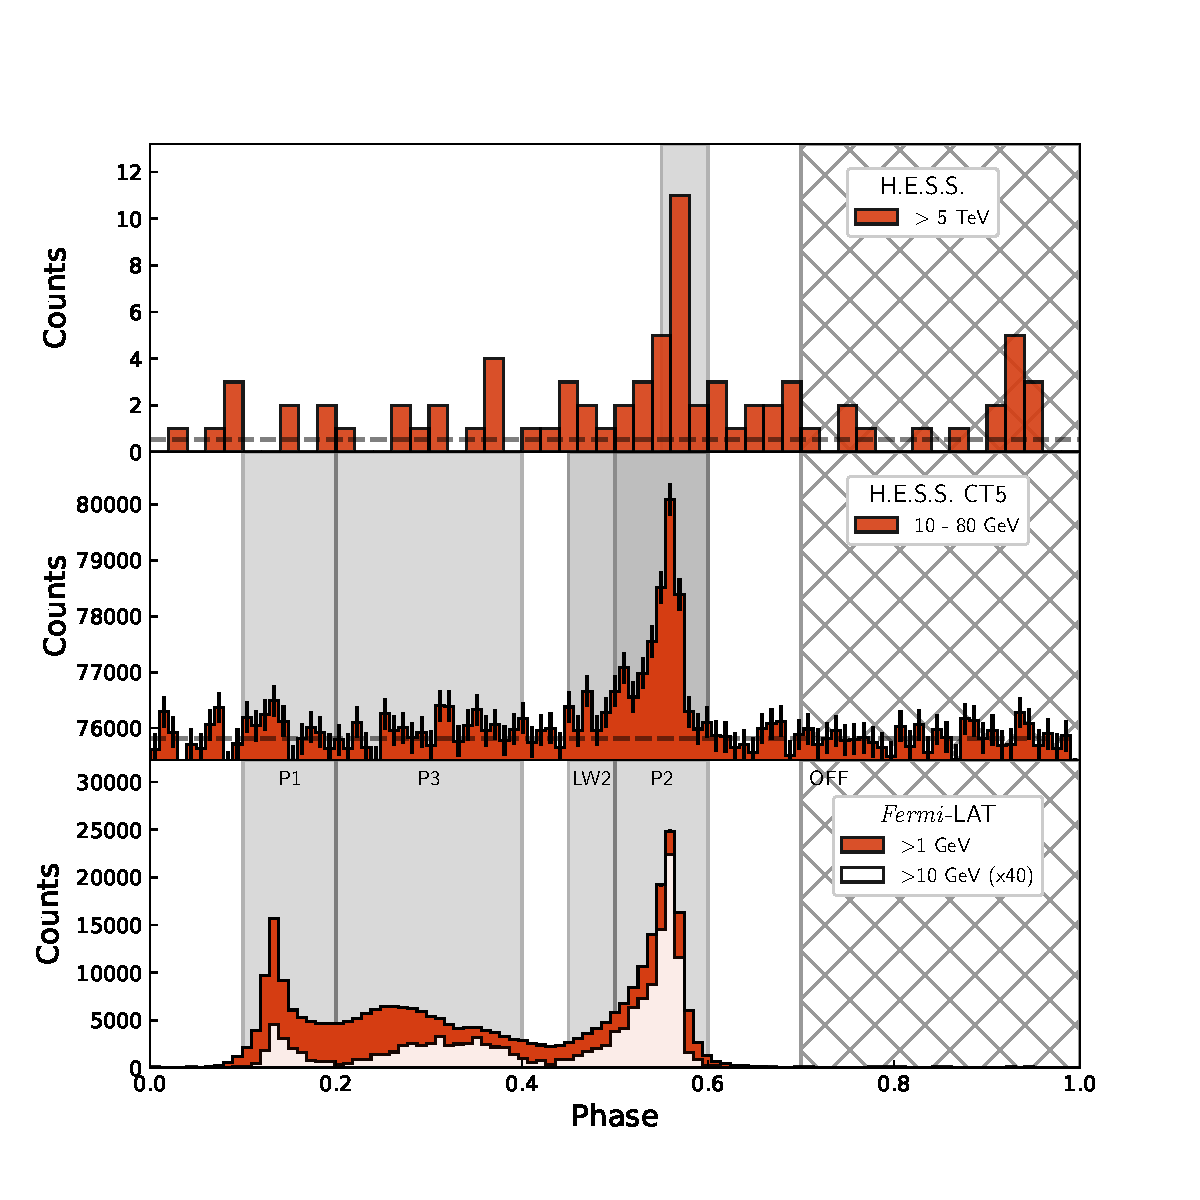
\includegraphics[
    width=0.80\textwidth,
    trim={0cm 0cm 0cm 13cm},
    clip
  ]{images/HESS_LAT_JointPhasogram_5TeV_v1.pdf}

  \vspace{0.03cm}

  {\scriptsize Vela pulse profile folded over one rotation period}

\end{frame}

\end{document}
